\section{MARCO TEORICO} 

\subsection{AZURE DATA STUDIO }
Azure Data Studio es una herramienta de base de datos multiplataforma para profesionales de datos que utilizan la familia de plataformas de datos en la nube y locales de Microsoft en Windows, MacOS y Linux.
\\Anteriormente publicado bajo el nombre de vista previa de SQL Operations Studio, Azure Data Studio ofrece una experiencia de edición moderna con IntelliSense, fragmentos de código, integración de control de fuente y un terminal integrado. Está diseñado teniendo en cuenta al usuario de la plataforma de datos, con un registro integrado de conjuntos de resultados de consulta y paneles personalizables.

\begin{center}
		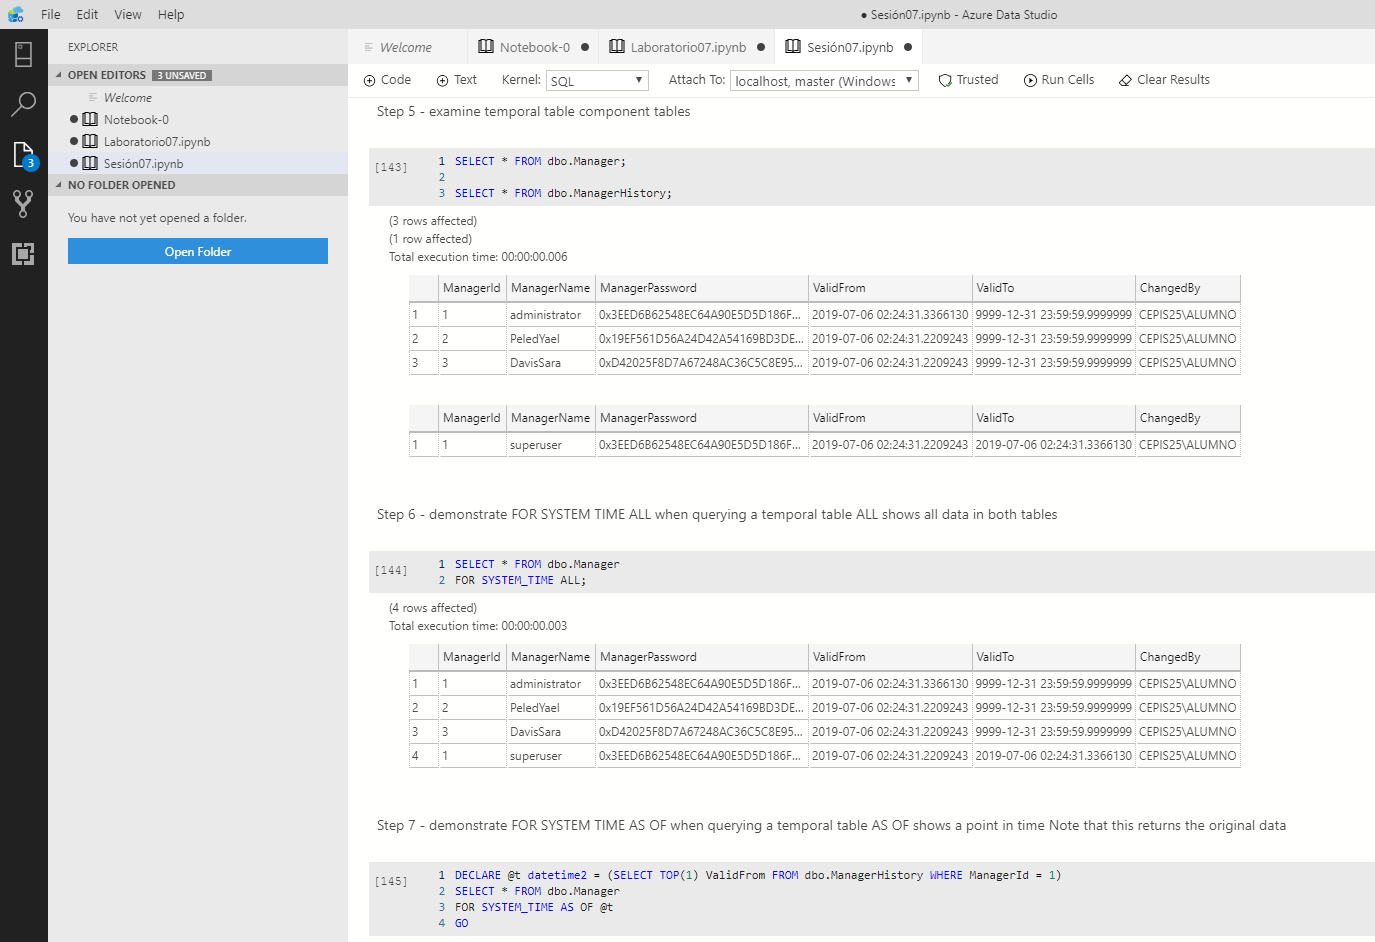
\includegraphics[width=15cm]{./Imagenes/1}
		\end{center}

\begin {itemize}
	\item Editor de código SQL con IntelliSense\\\\
	\subitem Azure Data Studio ofrece una experiencia moderna de codificación SQL centrada en el teclado que facilita sus tareas diarias con funciones integradas, como ventanas de pestañas múltiples, un editor de SQL enriquecido, IntelliSense, finalización de palabras clave, fragmentos de código, navegación de código y control de fuente integración (Git). Ejecute consultas SQL a pedido, vea y guarde los resultados como texto, JSON o Excel. Edite datos, organice sus conexiones de base de datos favoritas y explore los objetos de la base de datos en una experiencia familiar de búsqueda de objetos.
	\item Fragmentos de código de SQL inteligenter\\
	\subitem -Los fragmentos de código SQL generan la sintaxis SQL adecuada para crear bases de datos, tablas, vistas, procedimientos almacenados, usuarios, inicios de sesión, roles, etc., y para actualizar los objetos de base de datos existentes. Use fragmentos de código inteligente para crear rápidamente copias de su base de datos para fines de desarrollo o prueba, y para generar y ejecutar scripts CREAR e INSERTAR.\\\\
	\item Tableros personalizables de servidores y bases de datos\\
	\subitem -Cree ricos paneles personalizables para monitorear y solucionar rápidamente cuellos de botella de rendimiento en sus bases de datos. Para obtener información sobre los widgets de insight y los paneles de base de datos (y servidor), consulte Administrar servidores y bases de datos con widgets de insight .\\
	\item Gestión de la conexión (grupos de servidores)\\
	\subitem - Los grupos de servidores proporcionan una forma de organizar la información de conexión para los servidores y las bases de datos con las que trabaja. Para más detalles, consulte Grupos de servidores .\\\\
	\item Extensibilidad y autoría de extensión.\\
	\subitem - Mejore la experiencia de Azure Data Studio al ampliar la funcionalidad de la instalación básica. Azure Data Studio proporciona puntos de extensibilidad para las actividades de administración de datos, así como soporte para la creación de extensiones.\\
	
\end{itemize}





